\chapter{Background}

%5 pages minimum!, hopefully 8-10 though doubt it

%Section 1 on neural networks and how they work, CNNs, Alexnet, Inception (but no further)
\section{Neural networks}

%General theory for what a neural network is
%source to wikipedia here?
%Small figure showing what it looks like (simple neuron image thing)

\subsection{History}

%Rundown on nn history, 4 paragraphs
%p1: Early history, Hebb, backpropagation Werbos 1975

History of artificial neural networks used in computing can be traced back to its common roots with medicine and psychology that the NNs attempt to mimic. 
Towards the late 1940s, a book written by Donald Hebb \cite{hebb2005organization} describes the theory of how cells in a brain function together. 
As the brain cells fire electrical signals to other cells, those connections are strengthened and happen more frequently.
Artificial neural networks use this theory loosely to translate the signal received in the input neurons into proper outputs.
While the Hebbian theory allowed for the creation of first neural networks, these networks weren't very useful due to limitations in computing power and lack of more complex structures. 
Creation of deep neural networks with multiple layers was practically impossible until the creation of the backpropagation algorithm in 1975 by Paul Werbos\cite{werbos1975beyond}. 
Backpropagation allows for the errors to be sent back through many network layers, and adjust all of the weights in the network.

%p2: MOS-VLSI to create a practical network, max-pooling introduced in 1992, 90s-alexnet

Even with the creation of the backpropagation algorithm, the computational power of the time didn't allow for very complex neural networks. 
As execution in software was too difficult at the time, hardware solutions were created. Using the recent at the time metal-oxide semiconductors, in 1989 neural networks were implemented using very-large-scale integration in analog, rather than digital\cite{mead2012analog}. 
During the following two decades, various techniques were developed to enable neural networks to handle more complex problems.
Among others, max-pooling was introduced in 1992\cite{cresceptron1992}, and continuous improvement of existing and new technologies enabled neural networks to grow in relevance as more powerful hardware became available.

%p3: alexnet, non-commercial?, illustration of alexnet

The first in the series of convolutional neural networks that drastically improved the field of Artificial Intelligence is the deep neural network by Alex Krizhevsky \cite{Krizhevsky:2017:ICD:3098997.3065386}, created in 2012. 
%Deep layer technique, many layers stacked on top
A neural networks becomes "deep" when more than one layer is placed between the input and output layer.
AlexNet was constructed with five convolutional layers, followed by three dense layers, of which the last dense layer was the output layer.
In addition, several max pooling layers were placed throughout the model.
By using multiple convolutional layers in sequence, AlexNet managed to beat all of its competition that year in the ImageNet\cite{ImageNetMain} challenge\cite{ImageNet2012}. 


%p4: googlenet, commercial entity behind

After this breakthrough, commercial entities like Google used the findings in this paper to create the Inception\cite{szegedy2014going} network. 
This network utilized a combination of different convolutional layers in what it calls the Inception Module, seen in figure \cref{fig:inception}.
Unlike the previous models where one layer was strictly followed by the next layer, the Inception network has one-to-many and many-to-one connections that enable it to do multiple different operations on input from the same previous layer.
By combining the layers into building blocks, and then stacking them on top of each other, the first Inception NN beat out its competition in the 2014 challenge\cite{ImageNet2014}. %1-2 more sentences in the middle of this block
%


\begin{figure}[htbp]  % order of priority: h here, t top, b bottom, p page
  \centering
  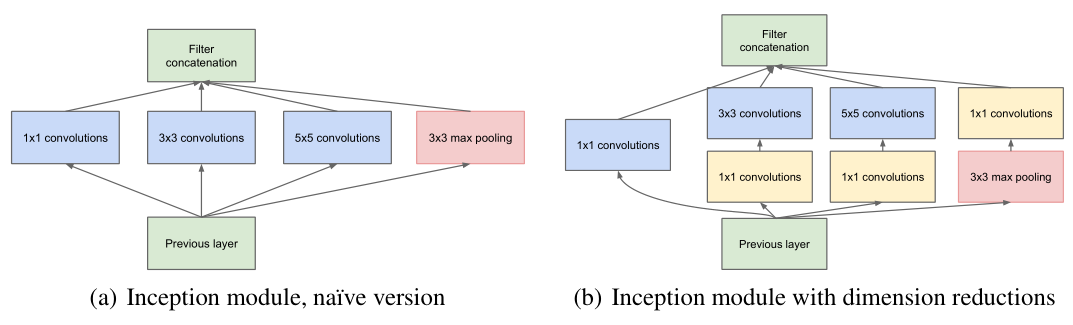
\includegraphics[width=.7\textwidth]{figures/google2.PNG}
  \caption{The Inception Module\cite{szegedy2014going}, without (left) and with (right) pooling layers in the module.}
  \label{fig:inception}
\end{figure}

\subsection{Convolutional neural networks}

%Rundown on what a CNN is, what it is used for
%Subsections for the direct explanation on the layers

%S0: dense layers, basic
\subsubsection{Dense layer}

%S1: conv layer (in particular the 1D version)
\subsubsection{Convolutional layer}

%S2: pooling layers, max and average
\subsubsection{Pooling layer}

%Custom images for all of this, but based on theory

%One more subsection tied to optimizers, loss functions and other stuff?
%Working title Gradient descent, uncertain if correct
\subsection{Gradient descent}
%Network needs to be trained to work, the process of adjusting this is (title of part)

\subsubsection{Optimizers}
%RMSProp, Adam (and variants), SGD?

\subsubsection{Loss functions}
%Categorical crossentropy

\subsubsection{Metrics}
%Loss number, accuracy

%Section 2 (probably earlier) on audio sample processing, what mfcc is, librosa
%Working title
\section{Audio processing}

\subsection{MFCC}

%1p about what MFCC is
%2 figures showing what mfcc is, dct 2 and 3
%1p explaining the difference?

\subsubsection{Applications}
%Pull some of the uses for mfcc papers here

%One more section on other ways to process audio, pick one of the options that were candidates later, cqt and the other maybe
\subsection{Other}

%Section 3 on trees, current existing methods of grouping data (agg, k-means etc)
%Working title, other can be 
\section{Hierarchical clustering}

%Explain the basics of clustering with the common one


%Explain the one used in the project
%Mostly stuff on current data clustering from scikit, but look for papers using this
%Basic rundown on hierarchical clustering
%NEEDS MORE SOURCES/LINKS
Among the current methods of clustering, hierarchical clustering is a relatively simple but powerful concept. Hierarchical clustering assumes that all data is in some way related to the rest of the dataset. The clustering process starts with assigning a score that represents the distance between each data point. Once the relationship is known, the data is clustered based on the score in one of two different ways. In the first method called «Agglomerative clustering,» the clusters are generated bottom-up, where each data point is its cluster, and the clustering aims to reduce the number of clusters by bringing close data points together. The second method, called «Divisive clustering,» starts with all data being in one cluster, dividing the data into smaller clusters recursively until the desired cluster number is reached.

%Bottom-up vs top-down
Each method of hierarchical clustering has its advantages and disadvantages. The most significant problem for the Agglomerative clustering is the significant performance penalty that requires processing the dataset multiple times. Some variations of the method can improve on this performance drawback to some extent. However, in general, the performance penalty comes from the exhaustive search and checking every possibility of improvement on the resulting clusters. Divisive clustering solves the problem of performance penalties by starting with one big cluster that is split recursively into smaller clusters. The most significant drawback is the potential for more optimal clusters to be available in the sub-clusters, as these will not be checked for potential merges by the algorithm.

%Used in Springer article, describe the article, mention relevancy in passing
One example of agglomerative clustering used in the processing of audio samples is found in an article about a modified dynamic tree warping method used in calculating distance between different audio samples\cite{ClusterExample}. The authors use agglomerative clustering to compare their modified DTW function with the standard, and then use two different scoring mechanisms to determine how well their function performed. For the two different scoring mechanisms, both top out at around 15 to 20 clusters. The number of clusters that the modified DTW method ended up giving the highest results for both scores is very relevant for the first master thesis research question of iterative training, as it serves as a foundation to base the initial cluster sizes on in the development of this thesis.


%Section 4 on how both tie together somewhat, use Tree-CNN as base and work up the chain in references
\section{Neural networks and data clustering}
%What Tree-CNN is and what it did
The concept of using neural networks in tree structures is not new. As NN layers learn information in a structured manner that focuses on more generic feature detection in the first layers, expanding these networks to become more hierarchical classifiers is possible. One example of this is Tree-CNN \cite{roy2018treecnn}, which in addition to using multiple models in its solution, also implements incremental learning that expands the capability of the model over time, rather than training it on the entire dataset at once.

%Section 5 on iterative training, use Tree-CNN paper here too?
\section{Iterative training}
%F
%Find papers that reference this, explain the concept


%Figures:
%Small net figure - visio
%conv operation - visio?
%pooling operation - visio?
%optimizer?
%MFCC sample graph - python
%cqt graph - python
%agg cluster picture - scikit
%tree-cnn picture of cluster from that report, maybe custom
%iterative training ill - custom, if no good source found on this